\documentclass{article}

\usepackage[T1]{fontenc}
\usepackage[utf8]{inputenc}
\usepackage[french,english]{babel}

%% This package is necessary to use \includegraphics.
\usepackage{graphicx}

%% This package is necessary to define hyperlinks.
\usepackage{hyperref}

%% These packages are necessary to include code.
\usepackage{listings}
\usepackage{minted} % colored

%% This package is needed to enchance mathematical formulas.
\usepackage{amsmath}

% This is a comment line in latex

% Latex allows you to define your own "commands",
% better known as "macros" in the Latex world.
% The following line is an example of such definition.
\newcommand{\latex}{\LaTeX}

% The next lines contain some meta informations about this document.

\title{Rapport intermédiaire de Projet long}
%\subtitle{A minimal demonstration of \latex}


\author{Mathieu Crocombette--Pasquet, Philippe Hinault}
\date{March 2024}

\begin{document}

\maketitle

\selectlanguage{french}

\section{Introduction}

Le but du projet est de faire un jeu de tactique militaire en temps continu, les règles du jeu sont détaillées dans le fichier rules.md (à la racine du projet).
La réussite du projet se mesure en évaluant à quel point le jeu est jouable, c'est à dire :

\begin{itemize}
\item L'interface graphique est-elle fonctionnelle ?
\item Les unitées peuvent-elles se déplacer / se battre / être posées sur le plateau ?
\item Le terrain peut-il être généré aléatoirement ?
\item Le jeu est-il fluide ? (moins de deux secondes entre chaque unité de temps)
\item Le jeu peut-il terminer ?
\item Un joueur peut-il affronter une IA ?
\end{itemize}

Nous réalisons le projet en Ocaml dans le but de monter notre niveau dans ce langage. Nous organisons notre travail en nous répartissant les tâches. Notre expérience pour ce projet se base sur des logiciels que nous avons déjà codés, soit : Un solveur de jeu solitaire (en Ocaml, avec lequel nous avons découvert le langage), un jeu Catane (en Java, où nous avons eu un plateau à gérer)

\section{Implémentation}

Notre code s'articule autour de modules dont le diagramme de dépendance correspond à la figure 1~\ref{fig:diagramme}

\begin{figure}
\label{fig:diagramme}
\hrulefill
\begin{center}
\includegraphics[height=200px,width=300px]{diagramme}
\end{center}
\caption{Diagramme module.}
\hrulefill
\end{figure}

\newpage

Nos données sont représentées sous forme de type record. Des tables de Hachage (Module Map) sont utilisées pour implémenter des files de priorité et des graphes.

Nous utilisons certaines librairies externes :

\begin{itemize}
\item LWT pour les threads.
\item YoJson pour la sérialisation
\item Raylib pour l'interface graphique
\end{itemize}

Notons que nous avons des difficultés pour utiliser les librairies LWT et Raylib en raison de la pauvreté de leur documentation en Ocaml. Aussi, la gestion d'erreur de Raylib est inexistante.

\section{Jalons}
Nous avons pris du retard sur le planning initialement prévu. Le nouveau planning est donc celui de la figure 2~\ref{fig:planning}

\begin{figure}
\label{fig:planning}
\hrulefill
\begin{center}
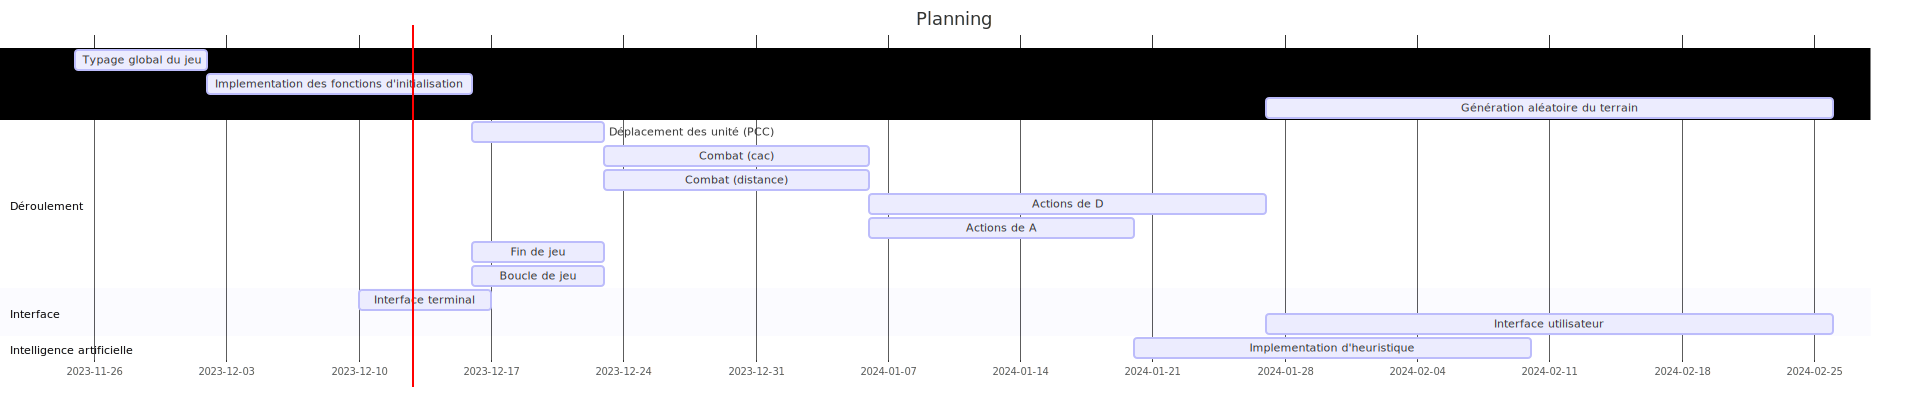
\includegraphics[height=200px,width=300px]{planning}
\end{center}
\caption{Planning.}
\hrulefill
\end{figure}

\newpage

\begin{description}

\item[Ce qui a été fait]: \\
- Les structures de données pour les pièces, les joueurs et le terrain\\
- L'affichage simple du jeu en interface graphique et terminal\\
- Les structures de communication entre l'interface et les contrôleurs du jeu\\

\item [Ce qui est en train d'être fait]:\\
- Les fonctions de parcours de graphe \\
- L'interface graphique

\item [Ce qu'il reste à faire]: \\
- La génération aléatoire du terrain (bruit de perlin) \\
- Les actions que peuvent faire les joueurs \\
- La boucle fluide du jeu \\
- L'implementation de l'IA \\
\end{description} 

\end{document}